\chapter{Refactoring}

\section{Code Smells} 

Im Folgenden sollen bekannte Code Smells im Code identifiziert werden. Im Abschnitt \hyperref[sec:Refactorings]{Refactorings} werden Refactorings beschrieben, die einige der Identifizierten Code Smells beheben sollen.


\subsection{Duplicated Code}
\label{sec:Duplicated_Code}

\textit{Duplicated Code} beschreibt, dass der gleiche beziehungsweise sehr ähnlicher Code an mehreren Stellen des Systems vorkommt.
Dadurch ist der Wartungsaufwand vergleichsweise hoch, da bei jeder Änderung potentiell mehrere Stellen angepasst werden müssen. Das kann auch dazu führen, dass sich die Funktionalität der einzelnen Stellen im Laufe der Zeit minimal unterscheidet, wodurch das Verhalten des Systems inkonsistent wird.
Um Duplicated Code zu reduzieren muss der doppelte Code ausgelagert werden und kann dann an verschiedenen Stellen wiederverwendet werden.
Die folgende Liste enthält Beispiele für Duplicated Code im vorliegenden Projekt.
Die meisten Stellen wurden bereits behoben.
\begin{itemize}
	\item{TimeSpanDetails: Click-Listener-Code wird vier mal in gleicher Form (bis auf eine Variable) verwendet. Gelöst mit {\hyperref[sec:ExtractMethod_TimeSpanDetails]{ExtractMethod}} bei Commit \href{https://github.com/lukaspanni/OpenSourceStats/commit/0c0b357dee742575d8465ae26e64152bfecbf5ab} {0c0b357}}
	
	\item{\textit{UserContributionRepository.userContributionsTimeSpan} und \textit{RepositoryDataRepository.repositorySummary} sind, bis auf die verwendeten Datentypen sehr ähnlich. 
Da beide Klassen von der gleichen Basisklasse erben wäre die Auslagerung einer Methode, in die Basisklasse eine denkbare Lösung.
\newline
Ein erster Schritt zur Verringerung des doppelten Codes ist durch das Refactoring {\hyperref[sec:ExtractMethod_Repository]{ExtractMethod}} bei Commit \href{https://github.com/lukaspanni/OpenSourceStats/commit/3b1eb5bf6750c3ccaeb05962ec8a8ae743adbf2c} {3b1eb5b} bereits umgesetzt.} 		
  \item{Der Konstruktor in \textit{ContributionCount} enthielt mehrere gleiche Codeteile, die in Commit \href{https://github.com/lukaspanni/OpenSourceStats/commit/34691d7b3b4bf00c483ce5c99d8e412f2732b6b1} {34691d7} beseitigt wurden}
  
  \item {Auch in der Klasse \textit{TimeSpanFactory} wurden mehrere Methoden gefunden, die zu Teilen aus dem gleichen Code bestehen. Dies wurde ebenfalls in Commit \href{https://github.com/lukaspanni/OpenSourceStats/commit/34691d7b3b4bf00c483ce5c99d8e412f2732b6b1} {34691d7} beseitigt.}
\end{itemize}
Durch die Code-Inspection von AndroidStudio konnten nicht alle der aufgeführten Dopplungen identifiziert wurden.
Mit Hilfe von IntelliJ IDEA Ultimate konnten weitere Dopplungen identifiziert und beseitigt werden.
Nach Beseitigung der genannten Dopplungen konnten mit der Inspection-Rule \textit{Duplicated code fragment} keine weiteren Dopplungen im Produktivcode gefunden werden.
Da nur wenige Dopplungen gefunden wurden und nur noch eine Kopplung weiterhin besteht, kann abschließend gesagt werden, dass der Code weitgehend frei von unnötigen Duplizierungen ist.

\subsection{Long Method \& Large Class}

Der Code Smell \textit{Long Method} zeichnet sich durch sehr lange Methoden aus, wobei die Länge, ab der eine Methode als zu lang betrachtet wird, von Projekt zu Projekt variabel sein kann.
Lange Methoden erschweren das Verständnis des Codes, was wiederum die Wartbarkeit und auch die Erweiterbarkeit einschränkt. 
Als Lösung kann die Lange Methode in mehrere kürzere Methoden aufgeteilt werden.
\newline
\newline
Ähnlich wie Long Method beschreibt \textit{Large Class}, Klassen, die vergleichsweise viele Code-Zeilen beinhalten.
Dies kommt häufig vor, wenn mehrere Verantwortlichkeiten in einer Klasse untergebracht werden. Auch hier kann die Verständlichkeit des Codes erschwert werden.
Das Aufteilen der Klasse in mehrere Klassen, ist eine sinnvolle Lösung für diesen Code Smell.
\newline
\newline
Um sowohl lange Methoden als auch große Klassen zu finden wurde das Code-Statistik Plugin \href{https://plugins.jetbrains.com/plugin/4509-statistic}{\textit{Statistic}} für Android Studio verwendet.
Um große Klassen oder Methoden zu finden, muss zunächst eine Obergrenze für die Methodenlänge fesgelegt werden.
Legt man zusätzlich eine maximale Anzahl von Methoden pro Klasse fest, lässt sich eine maximale Klassenlänge ableiten.
Im Buch \textit{Refactoring in Large Software Projects} wird angegeben, dass Methoden im Durchschnitt nicht länger als 30 Zeilen sein sollten \cite[p.~31]{refactoring_lippert}.
Außerdem wird beschrieben, dass eine Klasse weniger als 30 Methoden und damit auch weniger als 900 Zeilen umfassen sollte.
Die Längenvorgabe für Methoden soll auch hier verwendet werden.
Eine Klasse mit 900 Zeilen Code, ist aber meiner Meinung nach zu unübersichtlich für den praktischen Gebrauch.
Stattdessen sollte eine Klasse maximal etwa 200 Zeilen Code umfassen.
So kann der Code der Klasse noch schnell erfasst und verstanden werden und gleichzeitig wird eine zu starke Fragmentierung in viele einzelne Datein vermieden.
Aus diesem Grund sollen alle Klassen kleiner als 200 Zeilen Code sein.
\newline
Abbildung \ref{fig:class_length} zeigt die Länge der längsten Klassen im Projekt.
Keine der Klassen erreicht die maximale Anzahl an Zeilen.
Um die Länge der Methoden festzustellen wurden alle Klassen mit einer Länge von über 30 Zeilen untersucht.
Die Längste gefundene Methode besteht aus 28 Code-Zeilen und ist damit knapp kürzer als erlaubt.
\begin{figure}[h]
  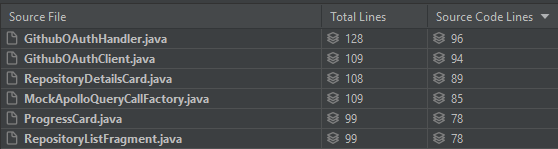
\includegraphics{class_length.png}
  \centering
  \caption{Größte Klassen des Projekts}
  \label{fig:class_length}
\end{figure}

\subsection{Shotgun Surgery}

\textit{Shotgun Surgery} beschreibt, dass für vergleichsweise kleine Funktionale Änderungen Anpassungen an vielen Stellen notwendig sind und deutet auf schlechte Struktur und eine Verflechtung von Verantwortlichkeiten hin.
Durch eine Umstrukturierung des Codes, sodass jede Klasse nur eine Verantwortlichkeit hat, kann dies behoben werden.
\newline
\newline
Dieser Code-Smell ist vergleichsweise schwer zu entdecken, wenn man danach sucht. Stattdessen kann dieser Code-Smell bei Anpassungen des Codes entdeckt werden.
Bisher wurde dieser Code-Smell bei keiner Änderung entdeckt.

\subsection{Switch Statements}

Die Verwendung von \textit{Switch Statements} fördert Fehler durch die unintuitive Syntax und verleitet oft dazu das gleiche Switch-Statement an mehreren Stellen einzusetzen.
Durch das übermäßige Verwenden von Switch Statements wird die Wartbarkeit und auch die Erweiterbarkeit des Codes eingeschränkt.
Switch Statements können in Objektorientiertem Code häufig durch die Verwendung von Polymorphie reduziert werden.
\newline
\newline
Im gesamten Code konnten keine Switch-Statements entdeckt werden. Außerdem wurde auch das Alternativkonstrukt (lange if-else Verkettungen) nicht entdeckt.

\subsection{Code Comments}

\textit{Code Comments} die beschreiben, was der Code an dieser Stelle tut, deuten häufig darauf hin, dass der Code an dieser Stelle unverständlich geschrieben ist.
\newline
\newline
Durch die Suche nach Kommentaren und eine Beurteilung der Kommentare in Bezug auf diesen Code-Smell ergab den folgenden Kommentar in den Klassen \textit{UserContributionsRepository} und \textit{RepositoryDataRepository}, der beschreibt, was der Code an dieser Stelle tut, was auf unverständlichen Code hindeutet.
\begin{lstlisting}
//Wrap callback to add response to cache
ClientDataCallback decoratedCallback = new ClientDataCallbackDecorator(callback, response ->  cache.put(repository, response));
\end{lstlisting}
Der Code an dieser Stelle ist ohne den Kommentar schwer verständlich. Um die Verständlichkeit des Codes zu erhöhen wurde das Refactoring {\hyperref[sec:ExtractMethod_Repository]{ExtractMethod}} bei Commit \href{https://github.com/lukaspanni/OpenSourceStats/commit/3b1eb5bf6750c3ccaeb05962ec8a8ae743adbf2c} {3b1eb5b} angewendet und die extrahierte Methode in die Basisklasse verschoben.


\newpage
\section{Refactorings}
\label{sec:Refactorings}

Die hier beschriebenen Refactorings sollen das Design des Systems verbessern, die Wartbarkeit und Erweiterbarkeit verbessern und auch die Verständlichkeit erhöhen.
Dadurch soll es unter anderem einfacher werden Fehler zu finden und zu beheben sowie neue Funktionen hinzuzufügen.


\subsection{ExtractMethod bei Commit \href{https://github.com/lukaspanni/OpenSourceStats/commit/0c0b357dee742575d8465ae26e64152bfecbf5ab} {0c0b357}}
\label{sec:ExtractMethod_TimeSpanDetails}

In der Klasse \textit{TimeSpanDetails} wurde sehr ähnlicher Code für einen Click-Listener an vier unterschiedlichen Stellen verwendet. Durch die Auslagerung in die Methode \textit{getClickListener}  kann der Duplicated Code vermieden werden. Durch die Einführung des Parameters \textit{resource} kann die extrahierte Methode flexibel an allen Stellen wiederverwendet werden. Dadurch wird außerdem die Lesbarkeit des Codes erhöht.
Auch eventuelle spätere Änderungen am Verhalten der Methode müssen so nur an einer Stelle durchgeführt werden.
\newline
\textbf{Code Vorher:} 
\begin{lstlisting}[breaklines=false]
[...]
view.findViewById(R.id.to_commit_repos)
    .setOnClickListener(v -> Navigation.findNavController(view)
    .navigate(R.id.action_1, getArguments()));
view.findViewById(R.id.to_issue_repos)
    .setOnClickListener(v -> Navigation.findNavController(view)
    .navigate(R.id.action_2, getArguments()));
[...]
\end{lstlisting}
\textbf{Code Nacher:} 
\begin{lstlisting}[breaklines=false]
[...]
view.findViewById(R.id.to_commit_repos)
    .setOnClickListener(getClickListener(view, R.id.action_1));
view.findViewById(R.id.to_issue_repos)
    .setOnClickListener(getClickListener(view, R.id.action_2));
[...]
\end{lstlisting}

\newpage
\subsection{ExtractMethod bei Commit \href{https://github.com/lukaspanni/OpenSourceStats/commit/3b1eb5bf6750c3ccaeb05962ec8a8ae743adbf2c} {3b1eb5b}}
\label{sec:ExtractMethod_Repository}

In den Klassen \textit{UserContributionsRepository} und \textit{RepositoryDataRepository} wurde doppelter und zusätzlich schlecht verständlicher Code verwendet. Um die Verständlichkeit des Codes zu erhöhen wurde eine Methode extrahiert und so benannt, dass die Funktion leicht verständlich ist. Die extrahierte Methode wurde in die Basisklasse verschoben, da diese Methode in allen Ableitungen der Basisklasse verwendet wird. Diese Änderung ist vergleichsweise klein erhöht jedoch die subjektive Verständlichkeit enorm.
\subsubsection*{Code Vorher:}
\begin{lstlisting}[breaklines=false]
ClientDataCallback decoratedCallback = new ClientDataCallbackDecorator(
	callback, 
	response -> cache.put(
		repository, (RepositoryDataResponse) response));
\end{lstlisting}
\subsubsection*{Code Nacher:}
\begin{lstlisting}[breaklines=false]
ClientDataCallback decoratedCallback = new ClientDataCallbackDecorator(
	callback, 
	getAddToCacheCallback(repository));
\end{lstlisting}

\newpage
\subsubsection{UML Vorher}
Abbildung \ref{fig:ExtractMethod_Refactoring_Before} zeigt das UML-Klassendiagramm vor dem Refactoring.
\begin{figure}[h]
  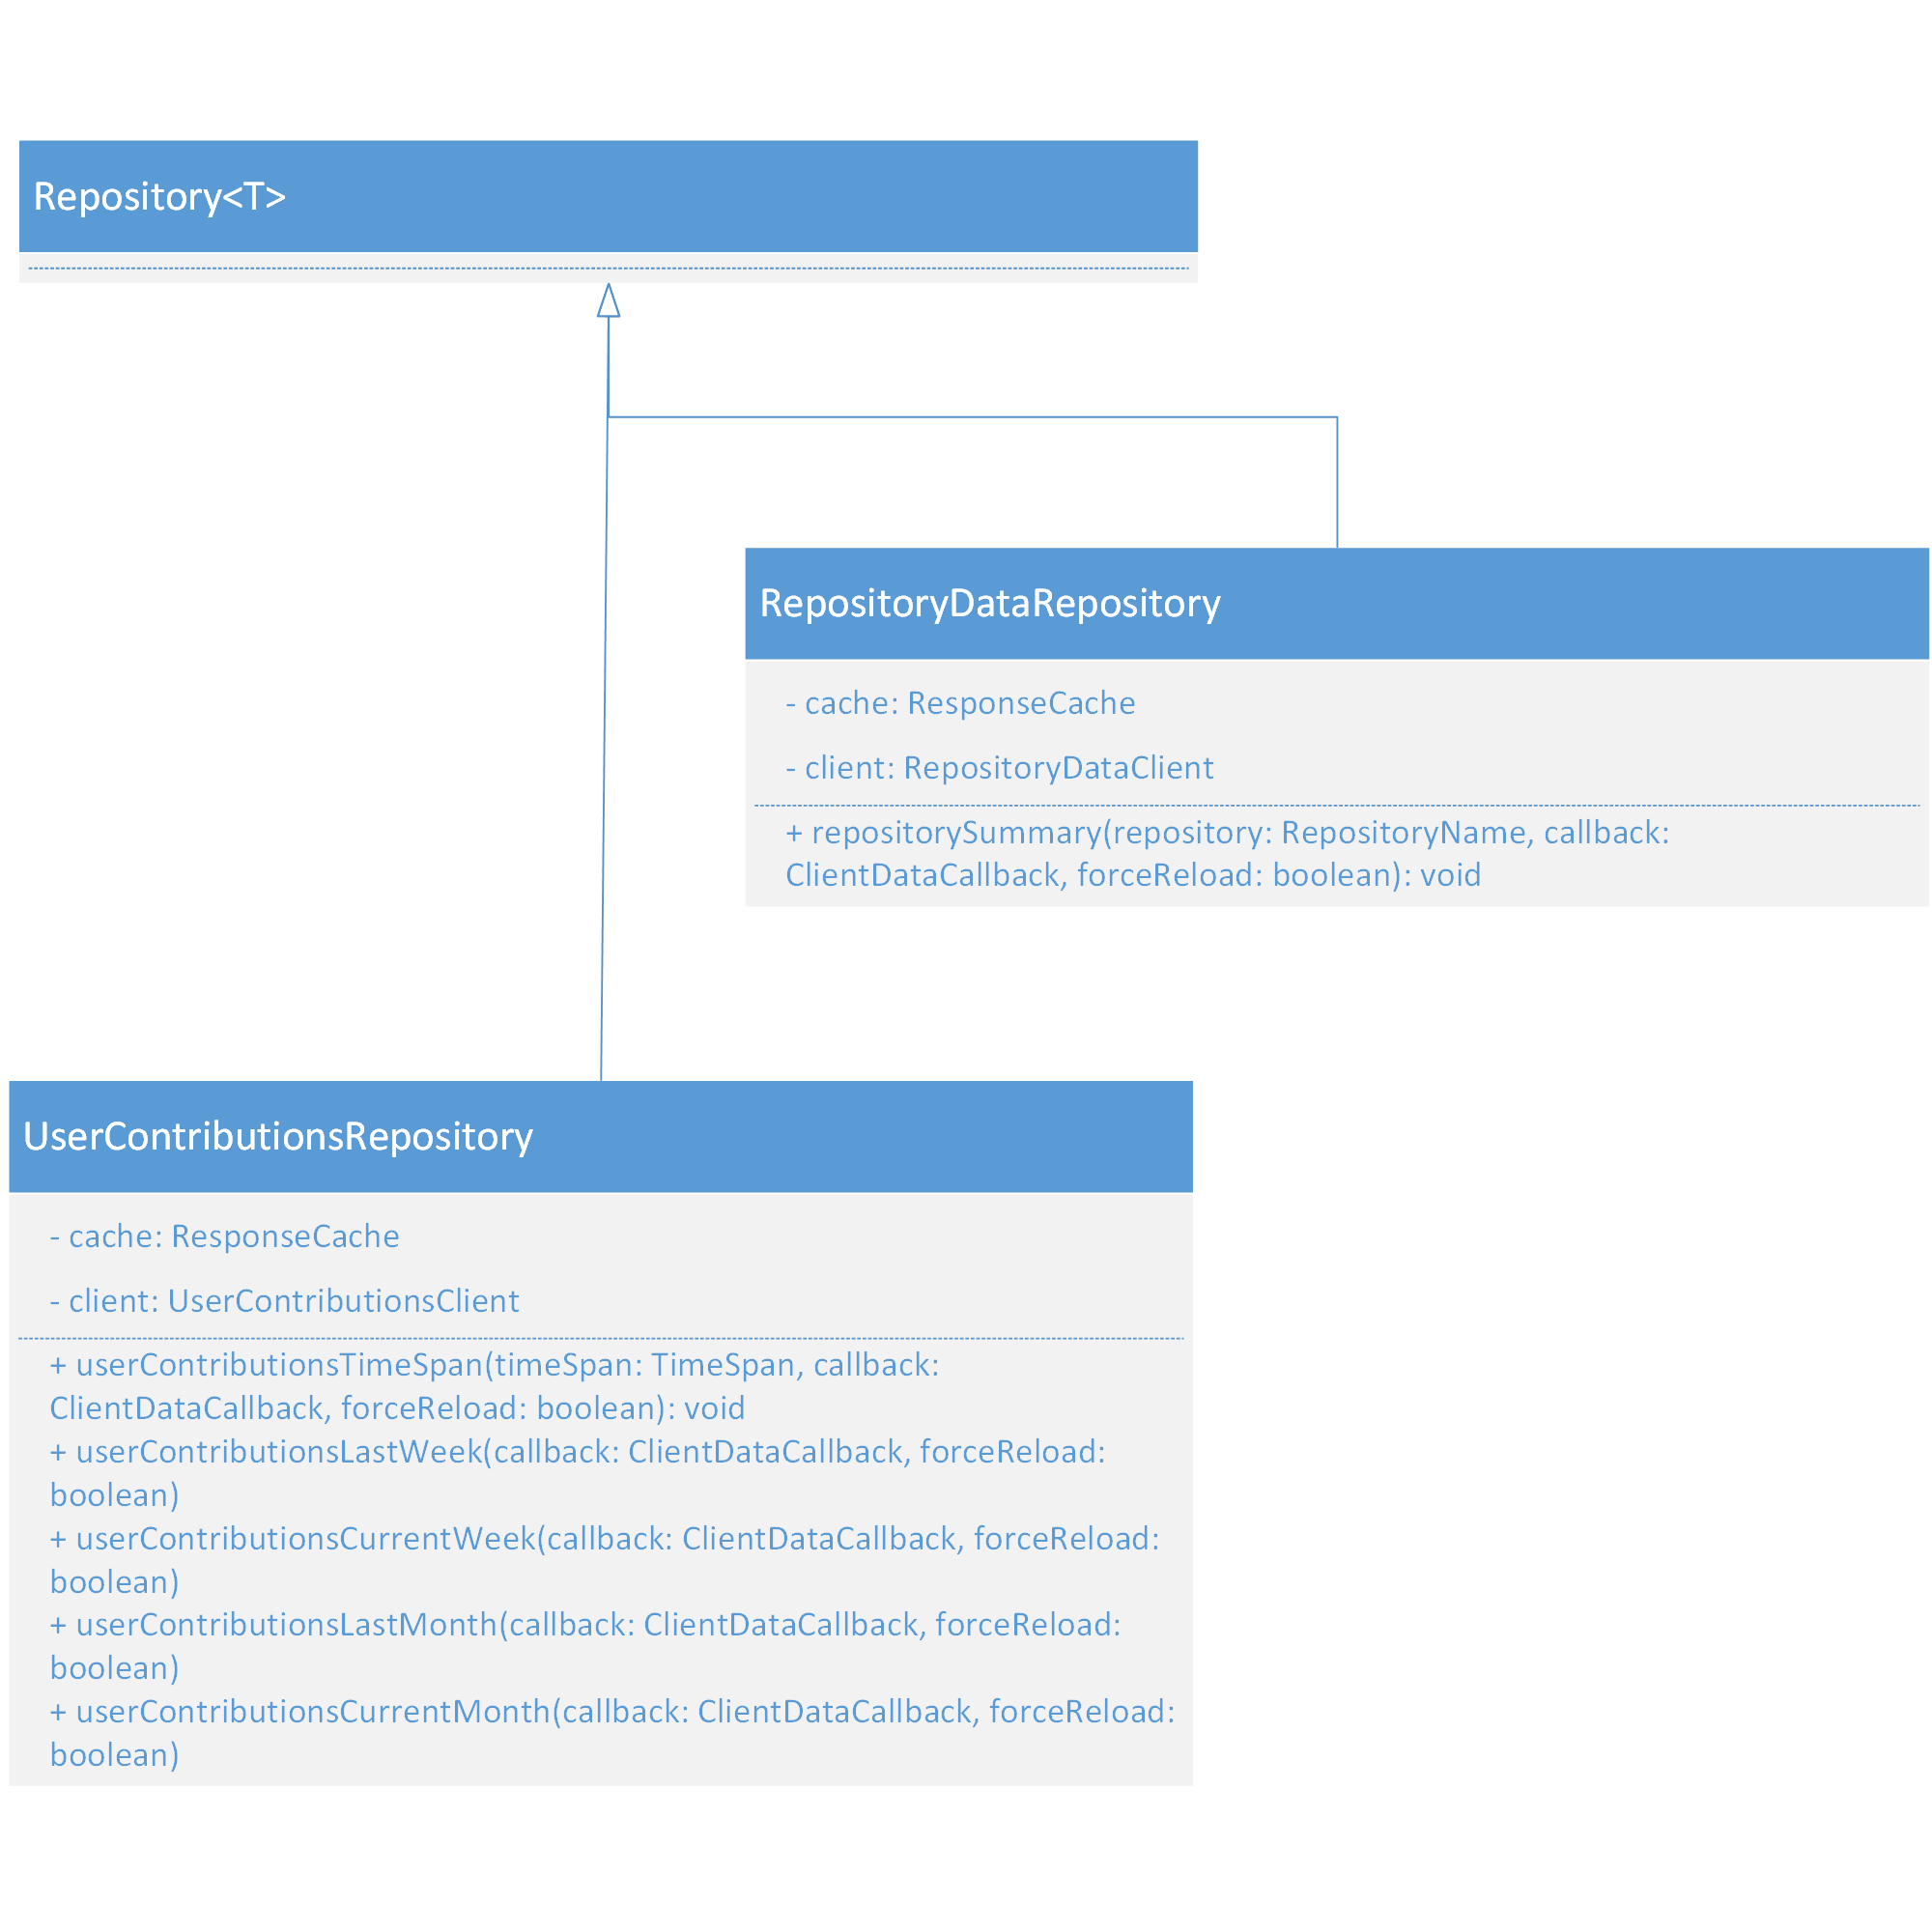
\includegraphics{refactoring_extract_method_repository_before.png}
  \centering
  \caption{UML vor Refactoring}
  \label{fig:ExtractMethod_Refactoring_Before}
\end{figure}

\newpage
\subsubsection{UML Nacher}
Abbildung \ref{fig:ExtractMethod_Refactoring_After} zeigt das UML-Klassendiagramm nach dem Refactoring.
\begin{figure}[h]
  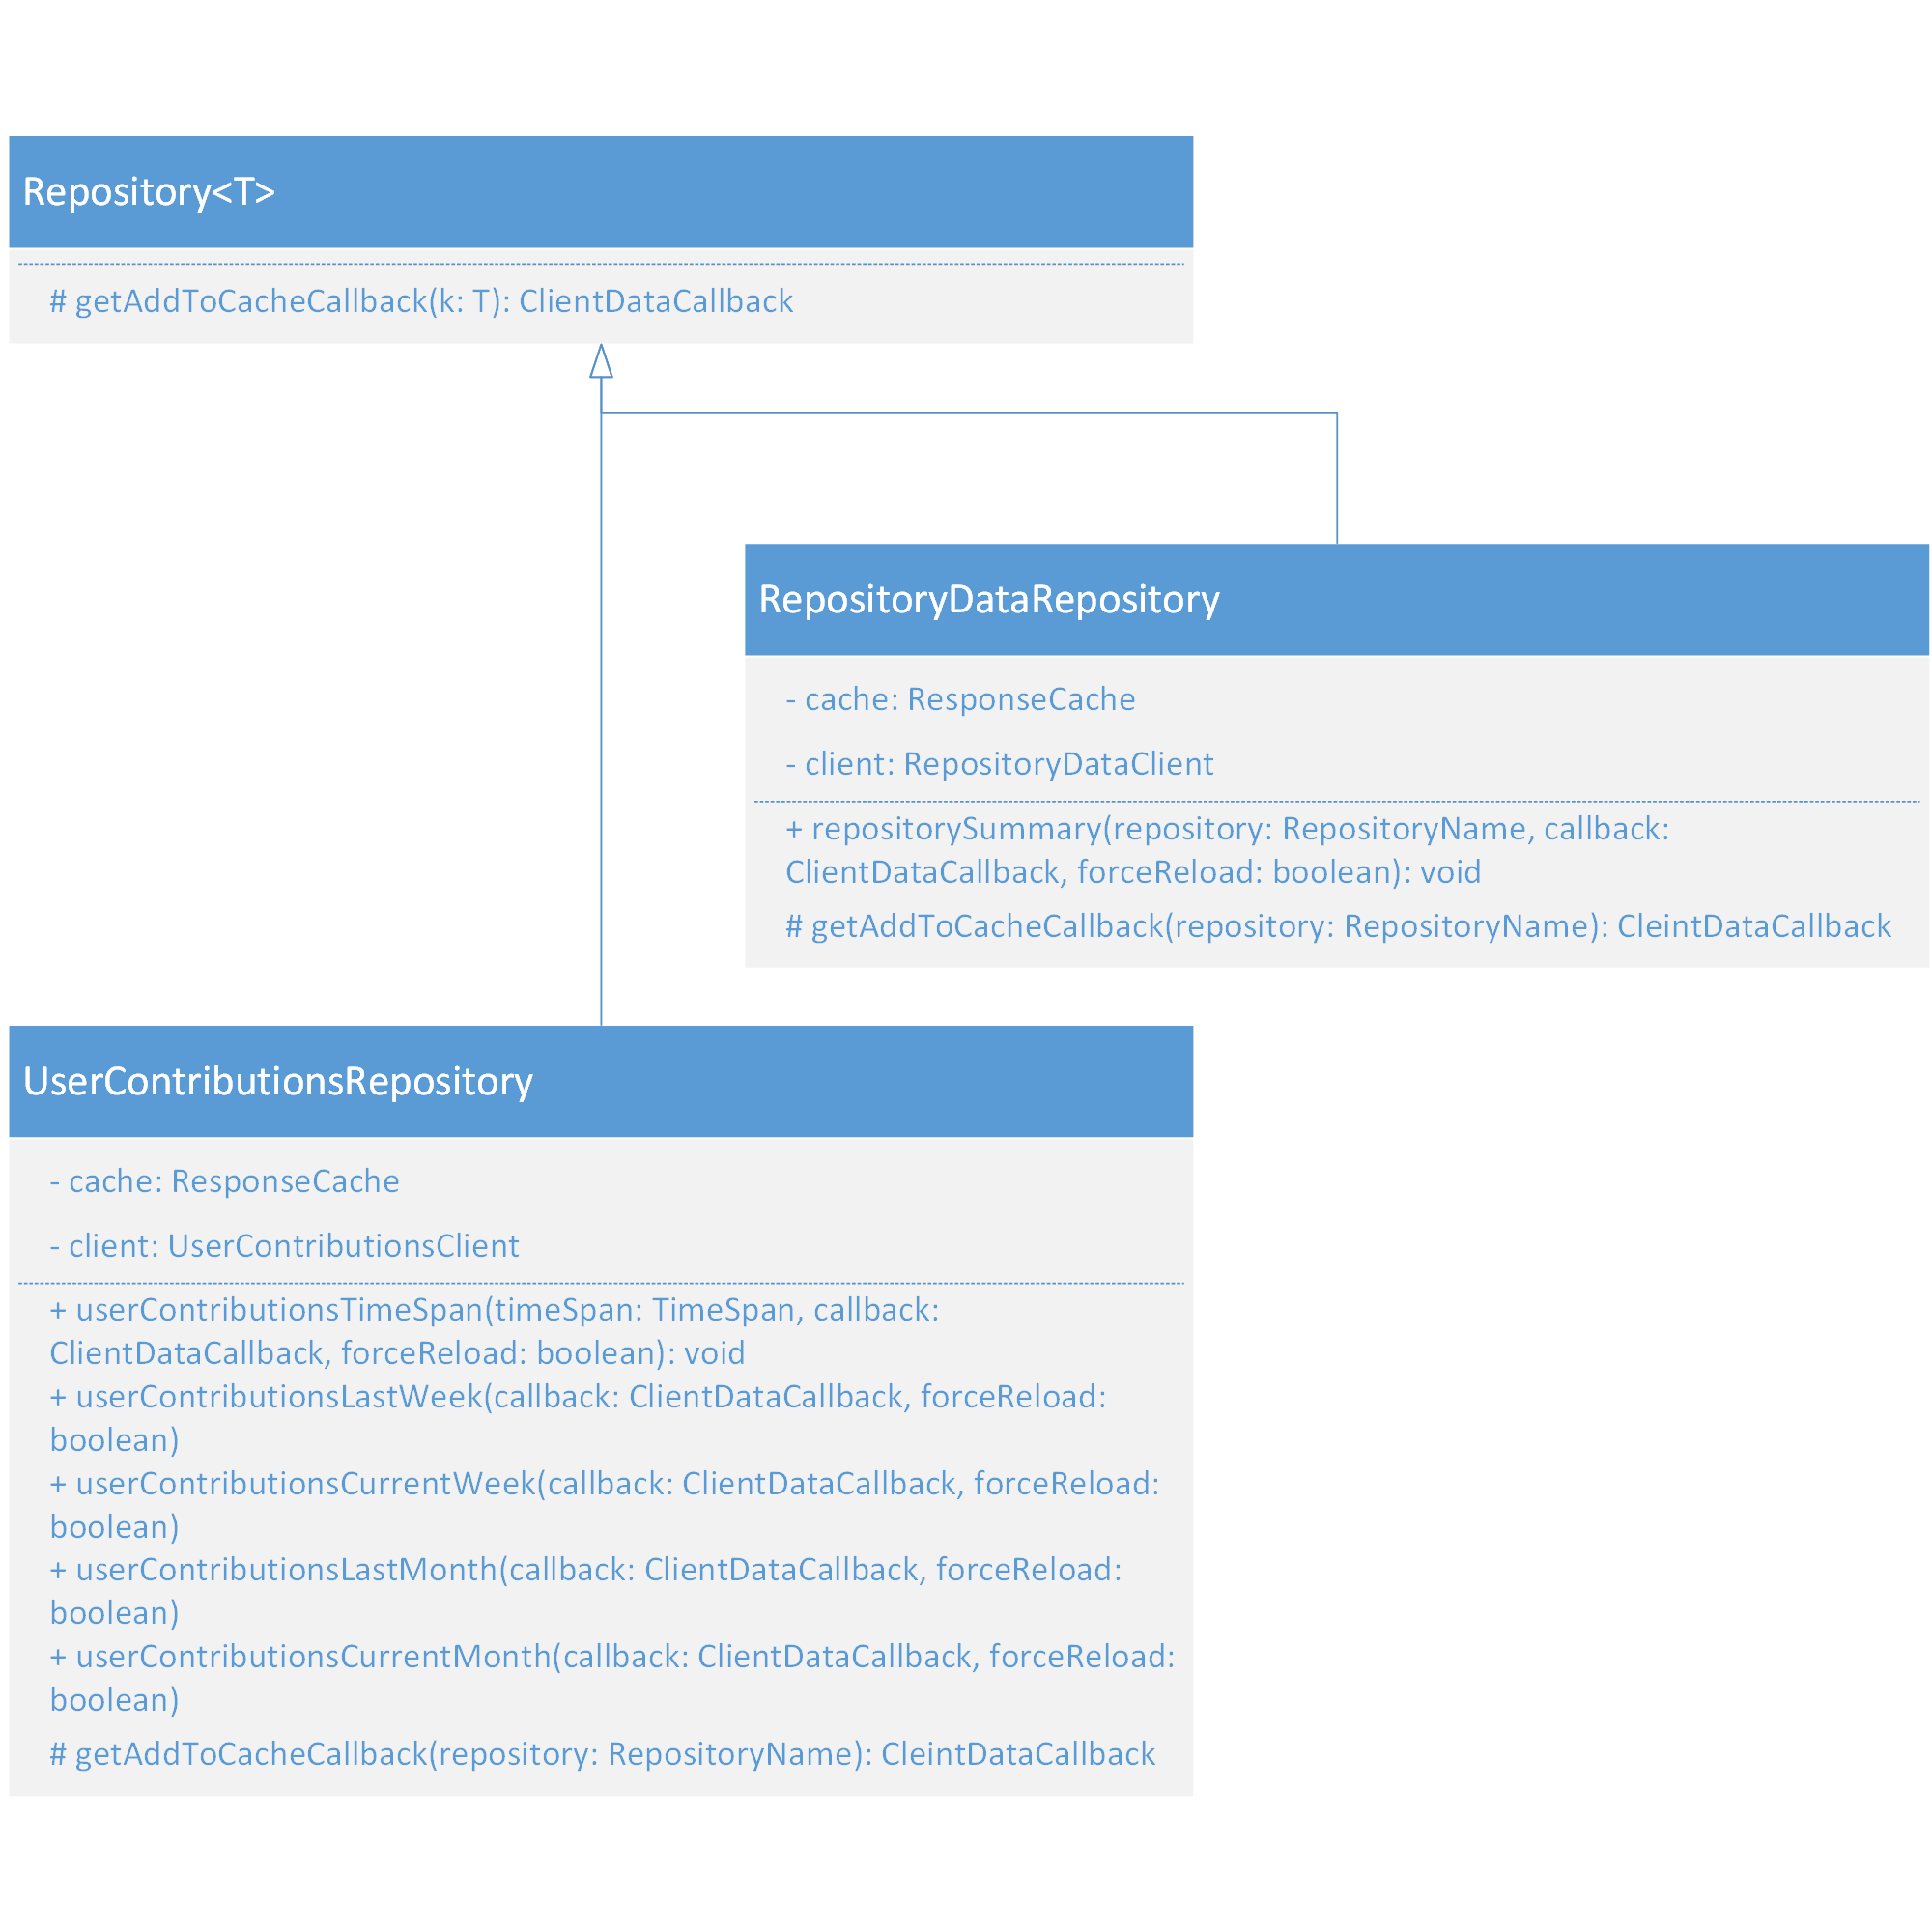
\includegraphics{refactoring_extract_method_repository_after.png}
  \caption{UML nach Refactoring}
  \label{fig:ExtractMethod_Refactoring_After}
\end{figure}
\newpage


\subsection{ExtractMethod bei Commit \href{https://github.com/lukaspanni/OpenSourceStats/commit/2eedf85be90e2566aa3811f9ccd3bac860c444a2} {2eedf85}}
\label{sec:ExtractMethod_AuthHandler}

Um die Singleton-Eigenschaft der Klasse \textit{AuthHandler} entfernen zu können, muss ein Teil der \textit{getInstance()} Methode in eine andere Methode übertragen werden.
Dafür wird das Refactoring \textbf{ExtractMethod} angewendet. So kann kann das Verhalten wiederverwendet werden. Teile des Verhaltens der \textit{getInstance()} Methode sind dadurch noch erhalten, auch wenn die ursprüngliche Methode in einem späteren Commit entfernt wird.


\subsection{RenameMethod bei Commit \href{https://github.com/lukaspanni/OpenSourceStats/commit/650235a5868f35cd0c641f0112b921ddead17a17} {650235a}}
\label{sec:RenameMethod_Repositories}

In den beiden Klassen \textit{RepositoryDataRepository} und \textit{UserContributionsRepository} werden Methodennamen verwendet, die den Zweck der Methode nur schwer verständlich machen. Um dies zu beheben wurde das Refactoring \textbf{ExtractMethod} angewendet.
\subsubsection*{RepositoryDataRepository}
Die Methode \textit{RepositoryDataRepository.repositorySummary} wurde umbenannt in \textit{RepositoryDataRepository.loadRepositoryData}, da dieser Name die Funktion der Methode deutlich besser beschreibt. Der alte Methodenname beschreibt nur den Zusammenhang mit einer Zusammenfassung über ein Repository, zeigt aber nicht deutlich genug, dass in dieser Methode Daten zu einem übergebenen Repository geladen werden. Auch war aufgrund des Methodennamens die Funktion des Parameters \textit{forceReload} unklar.
Mit dem neuen Methodennamen sollen der Code deutlich leichter verständlich sein.
\subsubsection*{UserContributionsRepository}
In dieser Klasse wurden mehrere ähnliche Methoden umbenannt:
\begin{itemize}
	\item{\textit{UserContributionsRepository.userContributionsTimeSpan} umbenannt in \textit{UserContributionsRepository.loadUserContributionsInTimeSpan}}
	\item{\textit{UserContributionsRepository.userContributionslastWeek} umbenannt in \textit{UserContributionsRepository.loadUserContributionsInLastWeek}}
	\item{\textit{UserContributionsRepository.userContributionsCurrentWeek} umbenannt in \textit{UserContributionsRepository.loadUserContributionsInCurrentWeek}}
	\item{\textit{UserContributionsRepository.userContributionslastMonth} umbenannt in \textit{UserContributionsRepository.loadUserContributionsInLastMonth}}
	\item{\textit{UserContributionsRepository.userContributionsCurrentMonth} umbenannt in \textit{UserContributionsRepository.loadUserContributionsInCurrentMonth}}
\end{itemize}
Wie bereits in der Klasse \textit{RepositoryDataRepository} soll der Code durch die Umbenennungen besser verständlich sein, indem die neuen Methodennamen die Funktion der Methoden besser beschreiben.
\newline
In Commit \href{https://github.com/lukaspanni/OpenSourceStats/commit/9385bb4b9e20b5503e3ea72acd392185f0c533db} {9385bb4} wurde zusätzlich eine Umbenennung in der Klasse \textit{GithubOAuthClient} vorgenommen um die Konsistenz zu den neuen Methodennamen der Klasse \textit{RepositoryDataRepository} zu steigern.
Konkret wurde die Methode \textit{GithubOAuthClient.repositoryData} zu \textit{GithubOAuthClient.loadRepositoryData} umbenannt. Durch diese kleine Änderung wird auch der Zusammenhang von \textit{GithubOAuthClient.loadRepositoryData} und \textit{RepositoryDataRepository.loadRepositoryData} besser deutlich.

\subsubsection{UML Vorher}
Abbildung \ref{fig:RenameMethod_Refactoring_Before} zeigt das UML-Klassendiagramm vor der Umbenennung der Methoden.
\begin{figure}[h]
  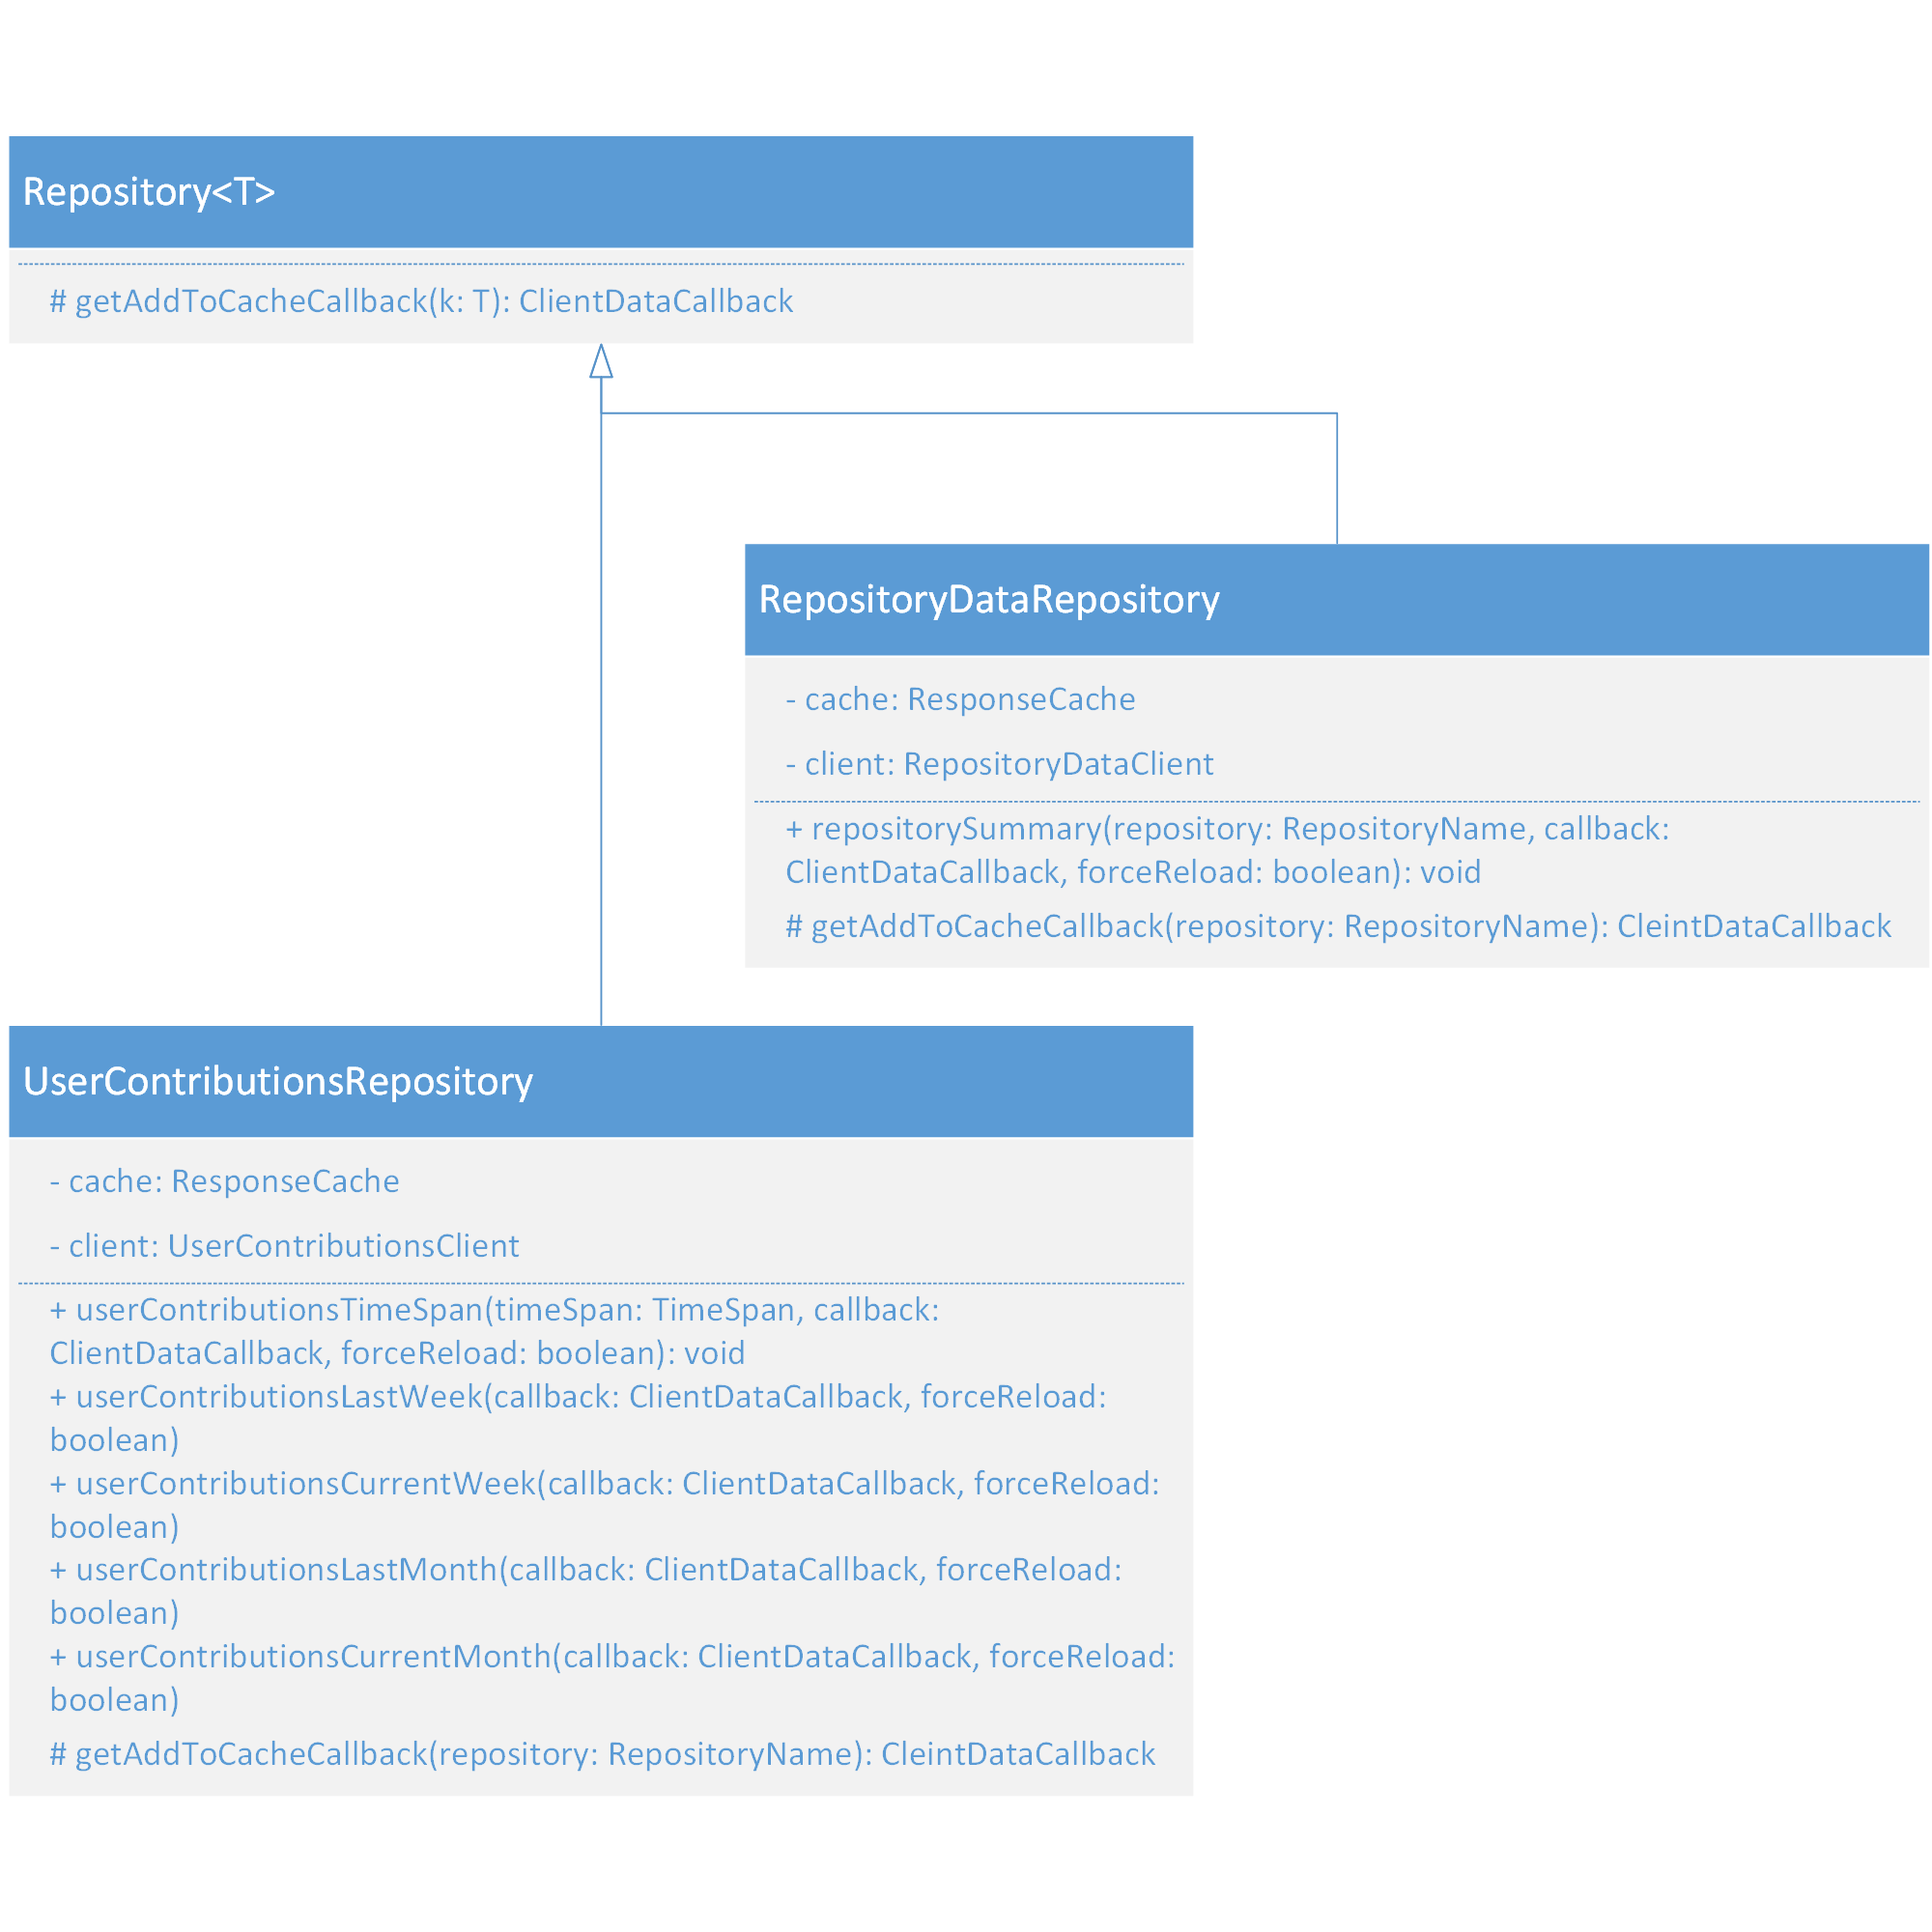
\includegraphics{refactoring_rename_method_repository_before.png}
  \centering
  \caption{UML vor Refactoring}
  \label{fig:RenameMethod_Refactoring_Before}
\end{figure}

\newpage
\subsubsection{UML Nacher}
Abbildung \ref{fig:RenameMethod_Refactoring_After} zeigt das UML-Klassendiagramm nach der Umbenennung der Methoden in \textit{UserContributionsRepository} und \textit{RepositoryDataRepository}.
\begin{figure}[h]
  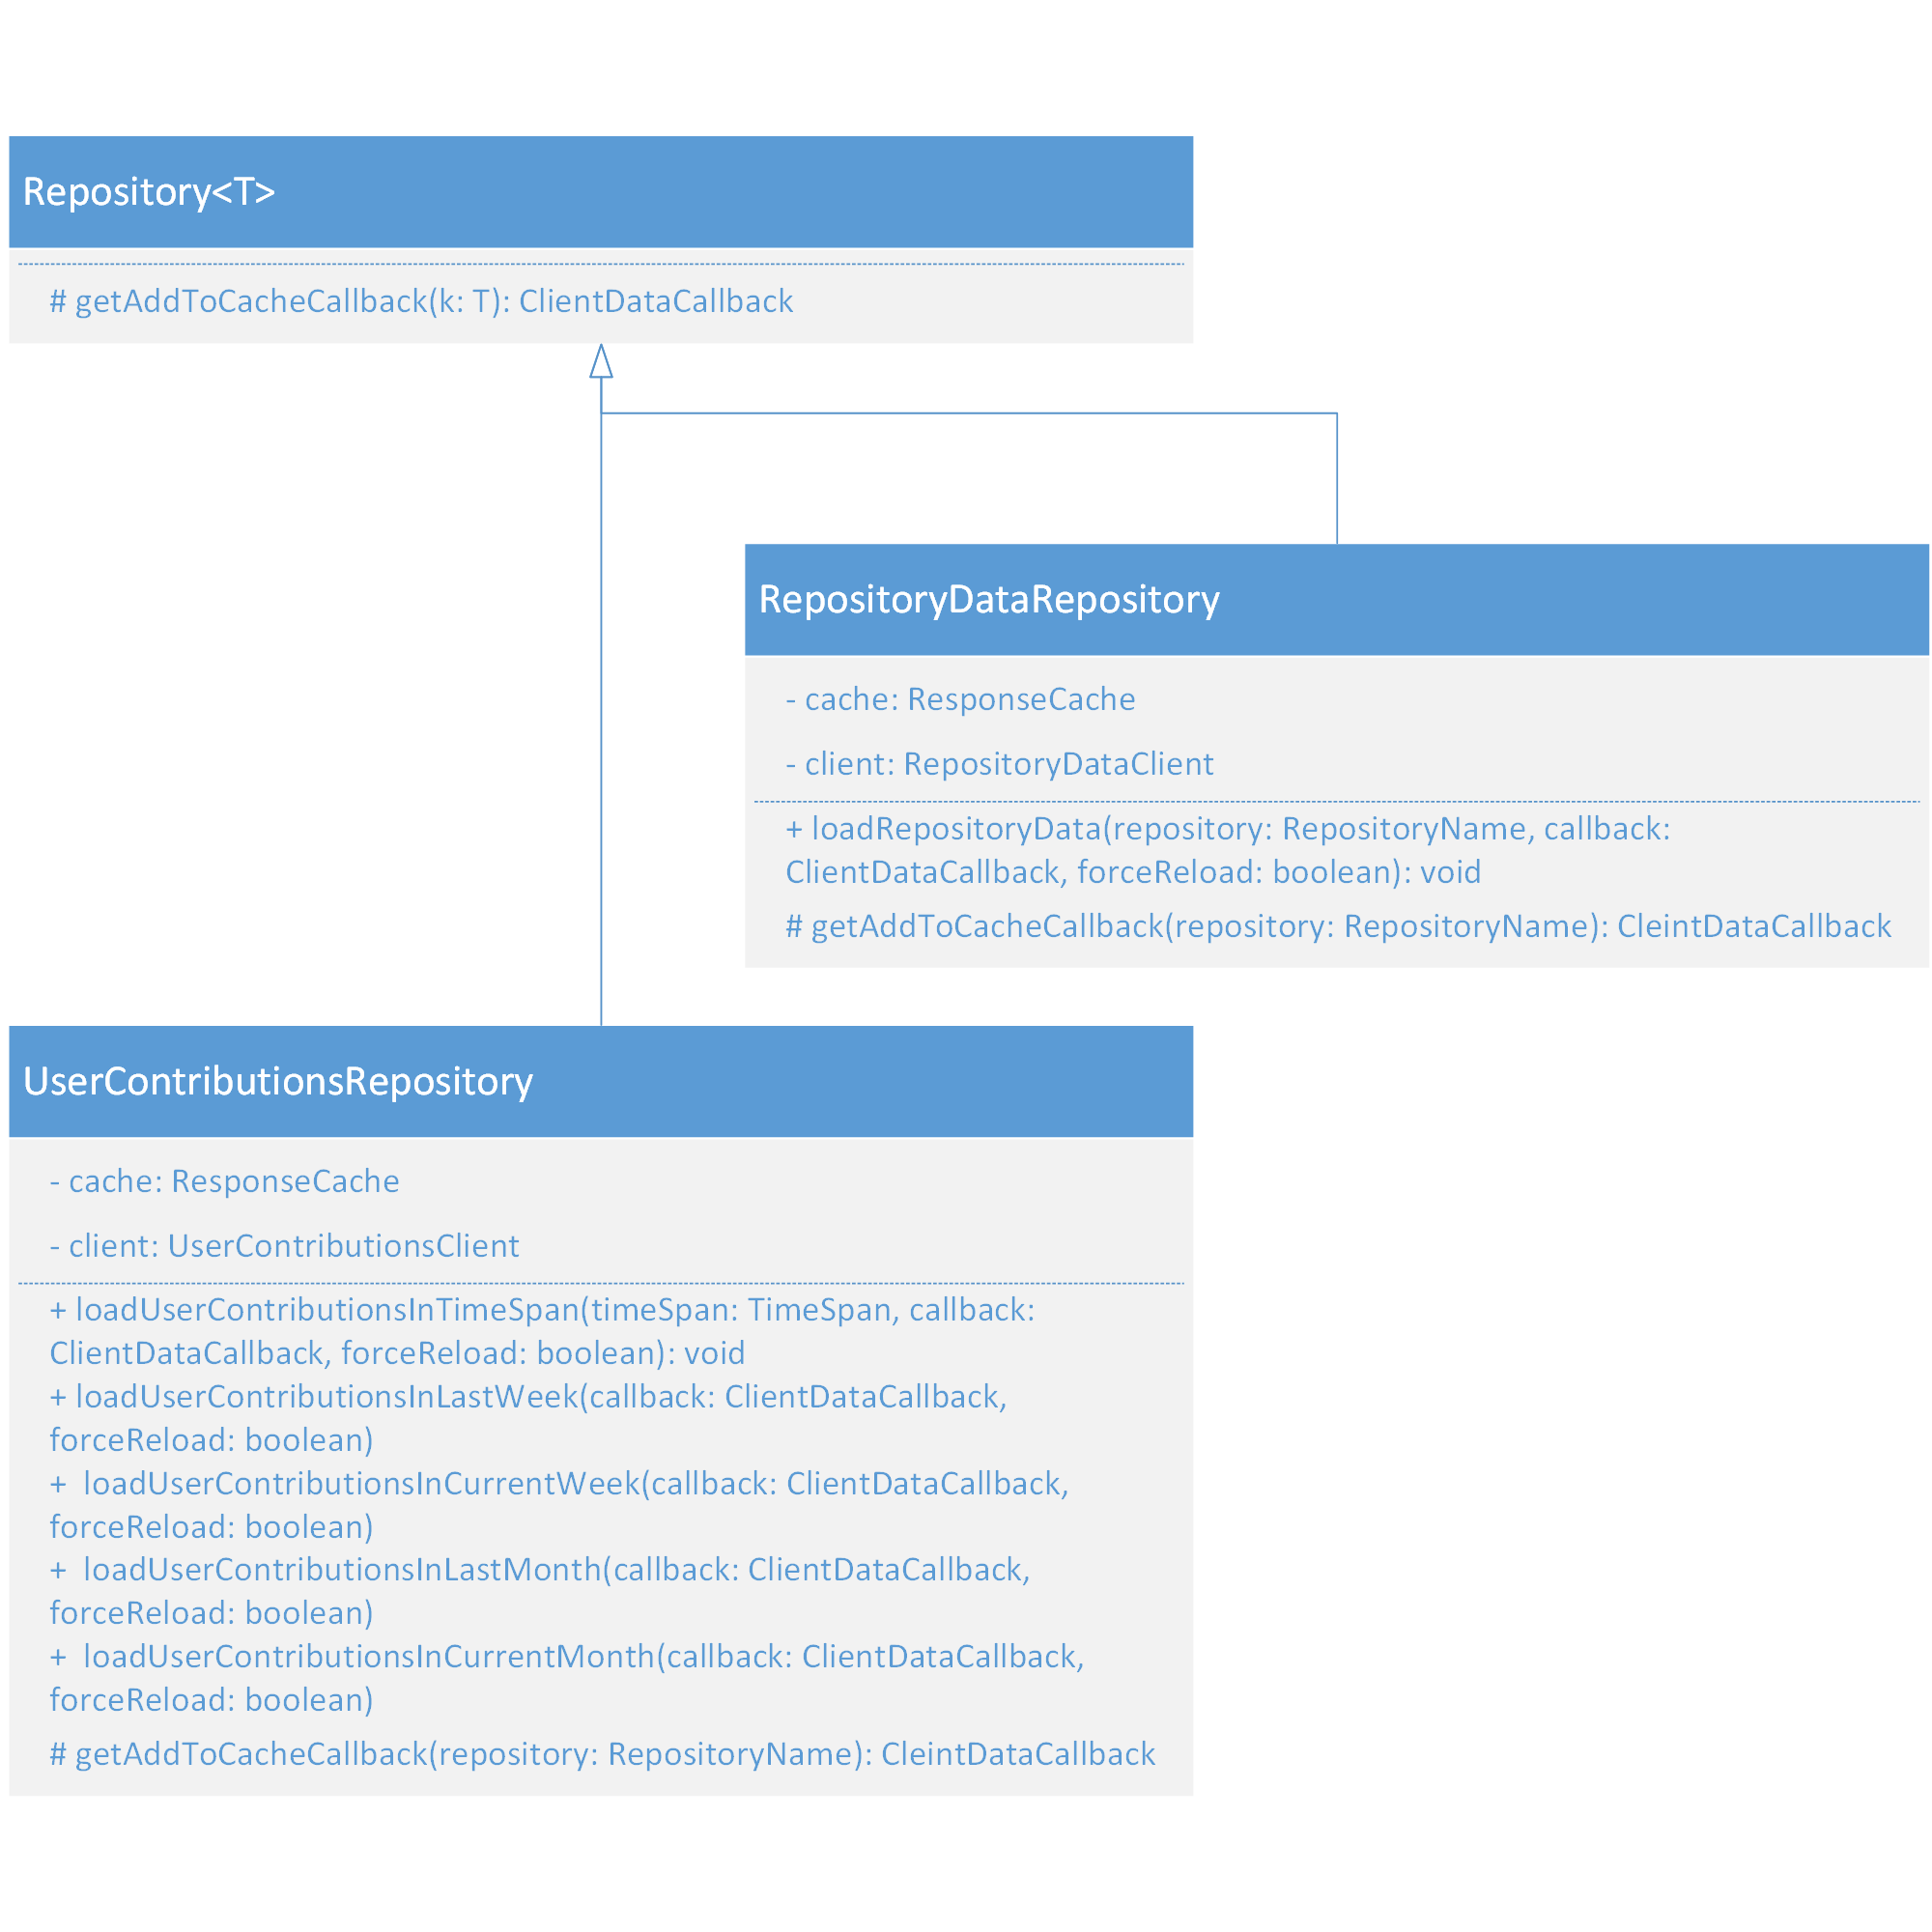
\includegraphics{refactoring_rename_method_repository_after.png}
  \caption{UML nach Refactoring}
  \label{fig:RenameMethod_Refactoring_After}
\end{figure}
\newpage